\cotefile{148}
\scanpage{44}
\mspage{1}
% archive sheet number: 43
\uline{Groupoïdes de Teichmüller.}

\textcircled{1} Cas topologique.

La variante la plus simple est
\[
\mathscr{T}_{\mathrm{top}}^{+}\quad\text{ou}\quad\mathscr{T}_{\mathrm{top}}
\]
(\uline{groupoïde de Teichmüller \uuline{orienté} topologique})

% slanted
\margin{Finalement, tant qu'on ne travaille pas au point de vue arithmétique, il semble que c'est le \unsure{gr.|gros} $\mathscr{T}^{\pm}$ qui \unsure{sera} le plus \unsure{utilisé}; \deleted{\unsure{tout}} c'est lui qui mérite donc ici la notation la plus simple $\mathscr{T}$, et le \unsure{gr.\ or.} orienté de s'appeler $\mathscr{T}^{+}$.}

\uline{Objts}: surfaces à \uline{bord} compactes orientées

\uline{flèches}: classes d'isotopie d'iso (conservant l'orientation)

Variante immédiate
\[
\mathscr{T}_{\mathrm{top}}^{\pm}
\]
(\uline{groupoïde de Teichmüller \uuline{biorienté} topologique}): mêmes objets, flèches sont les classes d'isotopie d'homéomorphismes (ne conservant pas \unsure{néc\textsuperscript{t}.|néc.} l'orientation).

Soit $[\pm1]$ le groupoïde ayant un seul objet $e$ (par exemple $e=\varnothing$) et comme groupe d'autom. $\pm1$. On a un morphisme de signature
\diagram{\begin{tikzcd}[ampersand replacement=\&]
\mathscr{T}_{\mathrm{top}}^{\pm}\arrow[r,"\chi"] \& {[\pm1]}
\end{tikzcd}}
dont la \uline{fibre} \deleted{est} (ou noyau) est $\mathscr{T}_{\mathrm{top}}^{+}=\mathscr{T}_{\mathrm{top}}$.

% slanted
\margin{\unsure{Cautèle}, \unsure{désormais borner} à des surfaces connexes !}

La variante la plus complexe est
\[
S_{*}\mathscr{T}\unsure{\mathbb{D}|D}_{\mathrm{top}}^{+}\quad\text{ou}\quad S_{*}\mathscr{T}\mathbb{D}_{\mathrm{top}},
\]
``\uline{groupoïde de Teichmüller \inserted{orienté} spécial dévissé topologique}''

\scanpage{45}
% archive sheet number: 44
\deleted{On a ainsi la notion de \uline{graphe pondéré} \uline{\unsure{enrichi}} (pondéré par $\unsure{\gamma|g}$, la structure}

\scanpage{46}
\mspage{2}
% archive sheet number: 45
\uline{Objets}: Triples $(X,\widetilde\Sigma,\deleted{\unsure{G|S}}\inserted{R})$, où

\margin{$X,\deleted{\unsure{\partial X}},\Sigma,S$}

$X$ surface à bord compacte orientée

$\widetilde\Sigma$ sous-$1$-variété compacte de $X\deleted{\unsure{\setminus\partial X}}$, $\widetilde\Sigma\supset\partial X$

$\deleted{\unsure{G|S}}R\subset\Sigma\deleted{\unsure{\setminus\partial X}}$, partie finie

% slanted
\margin{$\widetilde\Sigma=\partial X\amalg\Sigma$\par On peut considérer que $R$ rigidifie, \unsure{tandis} que $\deleted{R}\inserted{\widetilde\Sigma}$ ``découpe''\unsure{\ldots}}

\uline{flèches}: classes d'isotopie d'homéom. \inserted{conservant l'orientation}

\deleted{Variante} \deleted{\unsure{en}} Les compos. connexes de $\widetilde\Sigma\setminus\partial X\inserted{=\Sigma}$ sont les \uline{cercles de découpage}, \inserted{celles de $\partial X$ sont les cercles de \unsure{raccord|recollement}}; les éléments de $\deleted{\unsure{G|S}}R$ sont les \deleted{\unsure{points marqués}} \uline{sommets de \deleted{découpage}\inserted{rigidification}} \deleted{(ou de rigidification)}, \deleted{les composantes connexes de $\partial X$ sont les ``trous''}. Les composantes connexes de $X$ sont les \deleted{morceaux}\inserted{\uline{composants}} de l'objet envisagé.

Variante
\[
S_*\mathscr{T}\unsure{\mathbb{D}|D}_{\mathrm{top}}^{\pm},\quad\text{avec}
\]
\diagram{\begin{tikzcd}[ampersand replacement=\&]
S_*\mathscr{T}\mathbb{D}_{\mathrm{top}}\arrow[r,phantom,"\subset"] \& S_*\mathscr{T}\mathbb{D}_{\mathrm{top}}^{\pm}\arrow[r] \& {[\pm1]}
\end{tikzcd}}
comme tantôt.

On a des sous-groupoïdes pleins
\diagram{\[
\begin{array}{lll}
R=\varnothing,\ \Sigma=\deleted{\unsure{\partial X}}\varnothing & \mathscr{T}_{\mathrm{top}}\ \text{et}\ \mathscr{T}_{\mathrm{top}}^{\pm} & \\
\deleted{\unsure{G=\widetilde\Sigma=\varnothing}} & & \\
\Sigma=\deleted{\unsure{\partial X}}\varnothing & S_*\mathscr{T}_{\mathrm{top}}\ \text{et}\ S_*\mathscr{T}_{\mathrm{top}}^{\pm} & \text{(\unsure{groupoïdes|groupoïde} de Teichmüller} \\
\text{\inserted{$R$ quelconque}} & & \text{\uline{spéciaux}\inserted{ou \uline{rigidifiés}}} \\
& & \text{(topologiques \unsure{orientés|orienté}))} \\
\deleted{\unsure{G}}R=\varnothing & \mathscr{T}\mathbb{D}_{\mathrm{top}}\ \text{et}\ \mathscr{T}\mathbb{D}_{\mathrm{top}}^{\pm} &
\end{array}
\]}
(Cas pas intéressant je crois, sauf pour $\Sigma=\deleted{\unsure{\partial X}}\varnothing$ également)

% slanted
\margin{$\unsure{(MD)|MD}={}$``modulaire'' ou Mumford-Deligne}

\deleted{\unsure{Dé}} \uline{Détermination} du $\pi_0(S_*\mathscr{T}\mathbb{D}_{\mathrm{top}})\xrightarrow{\sim}\pi_0(S_*\mathscr{T}\mathbb{D}_{\mathrm{top}}^{\pm})$.

On introduit les \uline{graphes} \deleted{\unsure{MD}} bipondérés

\scanpage{47}
\mspage{3)}
% archive sheet number: 46
qui forment un groupoïde \deleted{\unsure{MD}} $\unsure{\mathrm{Grbip}|\mathrm{Grabip}}$ ou $(\mathrm{Grabipond})$

\uline{Objets}: graphes \inserted{finis} $(S,\vec A,\sigma,o)$ \inserted{$+$ structures suppl.}, (pouvant avoir des sommets isolés, des boucles fermées, a fortiori plusieurs arêtes entre deux sommets, et aussi des ``\uline{arêtes libres}'' correspondant aux pts fixes de $\sigma$) $S,\vec A$ ens. finis, $\sigma:\vec A\longrightarrow\vec A$ involution, $o:\vec A\longrightarrow S$ appl. ``origine''. On se donne de plus

% slanted
\margin{\unsure{pas assez précis}, comme \unsure{donnée} -- la pondération d'une arête doit être remplacée par celle d'un \unsure{pol.\ comb.} $T_a$ avec $\unsure{\omega(T_a)\simeq\omega(a)|\omega(T_a)\simeq\omega(0)|\omega(T_a)\simeq\omega(o)}$}
\inserted{(``sommets'', ``arcs'')}

\diagram{\begin{tikzcd}[ampersand replacement=\&]
S\arrow[r,"{\deleted{\unsure{g_0}}\unsure{\gamma|g}}"] \& \mathbb N
\end{tikzcd}}
(application ``genre'' ou ``poids'')

\margin{J'ai indiqué une pondération des sommets, mais pas des arêtes}
\figure{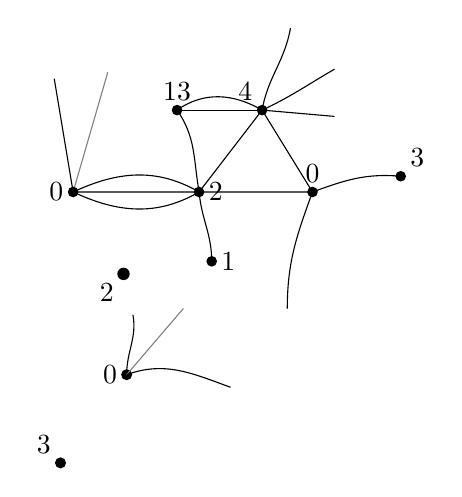
\begin{tikzpicture}[scale=.8]
\coordinate (a) at (0,2.8);\coordinate (b) at (2,2.8);\coordinate (c) at (3,4.1);\coordinate (d) at (1.65,4.1);\coordinate (e) at (3.8,2.8);\coordinate (f) at (5.2,3.05);\coordinate (g) at (2.2,1.7);
\draw (a)--(b)--(c)--(e)--(b);\draw (e) to[out=20,in=175] (f);\draw (b) to[out=-85,in=90] (g);\draw (d) to[out=-55,in=100] (b);\draw (d)--(c);\draw (d) to[out=35,in=150] (c);\draw (a) to[out=25,in=150] (b);\draw (a) to[out=-25,in=-150] (b);\draw (a) to[out=-120,in=260,looseness=6] (a);
\draw (a)--(-.3,4.6);\draw[gray] (a)--(.55,4.7);\draw (c) to[out=80,in=-100] (3.45,5.4);\draw (c) to[out=25,in=210] (4.15,4.75);\draw (c)--(4.15,4);\draw (e) to[out=-110,in=90] (3.4,.95);
\foreach \p in {a,b,c,d,e,f,g}{\fill (\p) circle (2.4pt);}
\node[left] at (a){$0$};\node[right] at (b){$2$};\node[above left] at (c){$4$};\node[above] at (d){$13$};\node[above] at (e){$0$};\node[above right] at (f){$3$};\node[right] at (g){$1$};
\fill (.8,1.5) circle (2.8pt);\node[below left] at (.8,1.5){$2$};
\fill (.85,-.1) circle (2.5pt);\node[left] at (.85,-.1){$0$};\draw (.85,-.1) to[out=90,in=-80] (.95,.85);\draw[gray] (.85,-.1)--(1.75,.95);\draw (.85,-.1) to[out=20,in=160] (2.5,-.3);
\fill (-.2,-1.5) circle (2.5pt);\node[above left] at (-.2,-1.5){$3$};\draw (-.2,-1.5) to[out=25,in=-25,looseness=7] (-.2,-1.5);
\end{tikzpicture}}

\diagram{\begin{tikzcd}[ampersand replacement=\&]
{\deleted{\unsure{\widetilde A}}\inserted{A_\ell}}\arrow[r,"{\inserted{r}\deleted{\unsure{\rho}}\unsure{r|2}}"] \& \mathbb N
\end{tikzcd}}
(application \deleted{\unsure{``multiplicité''}} ``indice de rigidification'')
\[
\deleted{\unsure{\widetilde A}\mathrel{\mathop{=}\limits^{\mathrm{def}}}\vec A/\sigma}
\]
\deleted{``\unsure{ens.\ des sommets apparents}''}

\deleted{Ou encore, posant $\widetilde S=S\amalg A_\ell$, (identif. à l'ens. de tous les ``sommets'' \inserted{apparents}, \deleted{\unsure{immergés}} et \inserted{``immergés'' (i.e. $\in S$)} les ``libres'', \inserted{\unsure{un correspondant à un $a\in A_\ell$}} du graphe), on donne}
\diagram{\begin{tikzcd}[ampersand replacement=\&]
\deleted{\widetilde S}\arrow[r,"\deleted{\pi}"] \& \deleted{\mathbb N}
\end{tikzcd}}
\deleted{(\uline{pondération} du graphe)}

\margin{$\widetilde S=S\amalg\deleted{\unsure{\widetilde S_\ell}}\inserted{A_\ell}$ \deleted{\unsure{sommets libres}}\par $\widetilde A=\vec A/\sigma=A\amalg A_\ell$}
\diagram{\begin{tikzcd}[ampersand replacement=\&]
\vec A\arrow[d]\& {=\vec A_0}\arrow[d,"\deg 2"]\arrow[d,phantom,shift left=5ex,"{\underbrace{\vec A\setminus\vec A^\sigma}}" description]\& {\amalg\vec A_\ell}\arrow[d,"\deg 1"]\arrow[d,phantom,shift left=5ex,"{\underbrace{\vec A^\sigma}}" description]\\
\widetilde A\& {=A}\& {\amalg A_\ell}
\end{tikzcd}}
\margin{Ordre d'un sommet\par $\sigma(s)=\underbrace{\sigma_\ell(s)}+\sigma_0(s)$\par \unsure{correspond} aux ``trous'' ou cercles de \unsure{recollage}}

La donnée du \uline{graphe} sous-jacent à un graphe \deleted{\unsure{MD}}\inserted{bip.} revient à celle d'un graphe ``ordinaire'' \unsure{accompagnant} (sans arêtes libres, i.e. $\sigma$ opère sans pts fixes), i.e.
\[
(S,(\vec A\setminus\vec A^\sigma),\sigma|_{(\vec A\setminus\vec A^\sigma)},o|_{\vec A\setminus\vec A^\sigma}),
\]
\uline{plus} un ensemble \inserted{fini} $A_\ell$ (\deleted{\unsure{``sommets''}}\inserted{arêtes} libres) \deleted{ou ``sommets-trous''} et une application
\diagram{\begin{tikzcd}[ampersand replacement=\&]
A_\ell\arrow[r] \& S
\end{tikzcd}}

\uline{Flèches} Les iso. de telles structures

\scanpage{48}
\mspage{4)}
% archive sheet number: 47
On a un foncteur
\[
\Gamma:\quad S_*\mathscr{T}\unsure{\mathbb D|D}_{\mathrm{top}}^{\pm}\longrightarrow\deleted{\mathrm{MD}}(\mathrm{Grabipond})\tag*{(*)}
\]
qui associe à un objet \inserted{$(X,\widetilde\Sigma,R)$} de $S_*\mathscr{T}\mathbb D_{\mathrm{top}}^{\pm}$ le graphe \inserted{MD} $(S,\vec A,\sigma,\deleted{\unsure{r|\rho}}\inserted{o},\deleted{\unsure{g}}\unsure{\gamma|g},\rho)$ suivant:
\[
S=\pi_0(X\deleted{\unsure{,}}\setminus\widetilde\Sigma)\simeq\pi_0(\mathrm{Déc}(X,\widetilde\Sigma))
\]
$\vec A={}$ ens des couples $(C,\deleted{\unsure{g}}\omega)$, où $C\deleted{\in A}\inserted{\in\pi_0}(\widetilde\Sigma)$, et où $\omega\in\mathrm{Or}(C)\inserted{\simeq\mathrm{rive}_X(C)}$, soumis à la condition que si $C\in\pi_0(\partial X)$, alors $\omega$ est l'orientation induite i.e. la rive qui se trouve dans $X$

$\sigma={}$ échange des rives (quand on a le droit d'échanger, sinon, i.e. si $C\in\pi_0(\partial X)$, on pose $\sigma(a)=a$)

$\deleted{\unsure{R|\rho}}\inserted{o}:{}$ associe à $(C,\text{rive de }C)$ l'unique ``\unsure{face}'' $\in\pi_0(X\setminus\widetilde\Sigma)$ qui contient cette rive

\[
\gamma:\underset{\Vert\atop\pi_0(X\setminus\widetilde\Sigma)}{S}\longrightarrow\mathbb N\qquad\text{application \uline{genre} des composants }X_i.
\]
\[
\unsure{r|\rho}:\quad A=\pi_0(\widetilde\Sigma)\longrightarrow\mathbb N:\quad C\longmapsto\mathrm{Card}(R\cap C).
\]

Le foncteur (*) \deleted{est \unsure{ess.} surjectif et}\inserted{induit un \uline{iso} sur les} $\pi_0$ et un surjectif sur les $\pi_1$ (c'est un \uline{$0$-isomorphisme}\deleted{\unsure{,}}, en langage homotopique).

\deleted{\unsure{Prop.}}:

\uline{\unsure{Remarque|Remarques}} Dans $S_*\mathscr{T}\mathbb D_{\mathrm{top}}^{\pm}$ il y a une opération évidente de \uline{somme} \inserted{\uline{discrète}}, dans \deleted{\mathrm{MD}}\inserted{$\mathrm{Grabipond}$} aussi, et (*) y commute.

\scanpage{49}
\mspage{5)}
% archive sheet number: 48
Cette opération de somme est la plus triviale parmi les opérations qu'il nous faudra expliciter et transcrire (combinatoirement) dans la suite. Notons de suite, pour $(X,\widetilde\Sigma,R)\deleted{\unsure{,}}$ donné
\[
X\deleted{\unsure{est}}\text{ connexe}\Longleftrightarrow\Gamma\mathrm{MD}(X,\widetilde\Sigma,R)\text{ connexe}
\]
plus précisément
\[
\pi_0(X)\simeq\pi_0(\Gamma\mathrm{MD}(X,\widetilde\Sigma,R))
\]
% slanted
\margin{\unsure{donner} la formule pour le genre d'un $\alpha\in\pi_0(X)\simeq\pi_0(\Gamma)$ en termes de la pondération -- plus généralement le \uline{genre total} est donné par $g=\sum_{s\in S}g_s+c(\Gamma)$\par $c(\Gamma)$: indice de connexion du graphe $=\deleted{\unsure{\mathrm{rg}}}\unsure{\mathrm{rg}\,H^1(\Gamma)|\dim H^1(\Gamma)}$}

\uline{Cas particuliers.}

a) Cas de $S_*\mathscr{T}_{\mathrm{top}}^{\pm}\deleted{\unsure{S_*\mathscr T_{\mathrm{top}}}}$ -- ici $\Sigma=\varnothing$, $\widetilde\Sigma=\partial X$.

Cela correspond aux graphes MD \deleted{qui} où \inserted{toutes les arêtes sont libres, i.e.} tous les sommets sont isolés (sauf arêtes libres) \deleted{\unsure{et}}\inserted{Graphe} est donc déterminé par
\diagram{\begin{tikzcd}[ampersand replacement=\&]
{A\ (\simeq\vec A=\vec A^\sigma)}\arrow[r,"r"]\arrow[d]\&\mathbb N\\
S\arrow[r,"\unsure{\gamma|g}"]\&\mathbb N
\end{tikzcd}}

Le cas de $\mathscr T_{\mathrm{top}}^{\pm}$ correspond à \unsure{admettre} $\rho=0$, donc la situation est donnée par
\diagram{\begin{tikzcd}[ampersand replacement=\&]
{A=A_0}\arrow[d]\&\\
S\arrow[r,"\gamma"]\&\mathbb N.
\end{tikzcd}}
\figure{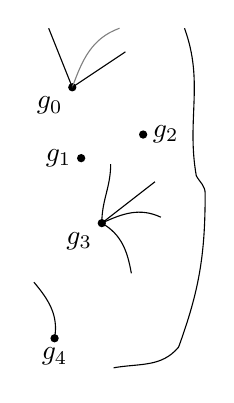
\begin{tikzpicture}[scale=.75]
\fill (0,3) circle (2pt);\node[below left] at (0,3){$g_0$};\draw (0,3)--(-.4,4);\draw[gray] (0,3) to[out=70,in=200] (.8,4);\draw (0,3)--(.9,3.6);
\fill (.15,1.8) circle (2pt);\node[left] at (.15,1.8){$g_1$};\fill (1.2,2.2) circle (2pt);\node[right] at (1.2,2.2){$g_2$};
\fill (.5,.7) circle (2pt);\node[below left] at (.5,.7){$g_3$};\draw (.5,.7) to[out=90,in=-90] (.65,1.7);\draw (.5,.7)--(1.4,1.4);\draw (.5,.7) to[out=25,in=155] (1.5,.8);\draw (.5,.7) to[out=-30,in=100] (1,-.15);
\fill (-.3,-1.25) circle (2pt);\node[below] at (-.3,-1.25){$g_4$};\draw (-.3,-1.25) to[out=80,in=-50] (-.65,-.3);
\draw (1.9,4) to[out=-70,in=100] (2.1,1.5) to[out=-60,in=90] (2.25,1.2) to[out=-90,in=70] (1.8,-1.4) to[out=-130,in=10] (.7,-1.75);
\end{tikzpicture}}

Le cas d'une structure connexe ($\mathrm{Card}.S=1$\inserted{i.e. $S=\{s\}$}) \deleted{type $(g,\nu)$ d'une structure} est \deleted{\unsure{déterminé par le genre}}\inserted{caractérisé} par la donnée des deux entiers $(g,\nu)$ ($g={}$genre, $\nu={}$nb de trous)
\[
g=\gamma(s),\quad\nu=\mathrm{card}\,A
\]

\scanpage{50}
\mspage{6}
% archive sheet number: 49
\uline{Remarque} En fait, on a un foncteur plus précis, vers une catégorie de graphes munis d'une structure où la partie $\rho$ de la pondération est \deleted{complétée}\inserted{remplacée} par une structure plus précise, à savoir \deleted{une application}\inserted{une \deleted{\unsure{appl.}} famille}
\[
\deleted{\unsure{A}\ (\widetilde R,\alpha,p:R\longrightarrow\underset{\Vert\atop\vec A/\sigma}{\vec A})}\quad(R_a)_{a\in A}
\]
d'ensembles, et pour $\forall a\in A$, si $\omega(a)$ désigne l'ens. des ``orientations'' de $a$ ($\mathrm{card}(\omega(a))\in\{1,2\}$), une application

% slanted
\margin{$\omega(a)\mathrel{\mathop{=}\limits^{\mathrm{def}}}\{\vec a\in\vec A\mid\vec a\text{ au-dessus de }a\}$}

\deleted{\unsure{$R$ est un ens. fini muni d'une involution de} $R$, et $p$ une application $R\longrightarrow A$ \unsure{compatible à $\alpha$}}
\[
\omega\longmapsto u_\omega:\quad\omega(a)\longrightarrow\mathrm{Circ}(R_a)
\]
ens des permutations circulaires sur $R_a$

\deleted{et induisant une \unsure{bij.} une application \unsure{injective}}
\[
\deleted{R/\alpha\longrightarrow\vec A}
\]
sous la condition que si $\omega,\omega'\in\omega(a)$, $\omega\ne\omega'$, alors $\deleted{u_\omega u_{\omega'}=\mathrm{id}_R}\ u_{\omega'}=u_\omega^{-1}$.

On peut aussi considérer que la donnée des \unsure{suppléments|supplémentaires} revient à la donnée de
\[
\begin{aligned}
r:&\quad A\longrightarrow\mathbb N\\
&\quad a\longmapsto\mathrm{Card}\,p^{-1}(a)
\end{aligned}
\]
(la ``pondération-arêtes''), et la donnée d'une famille de torseurs
\[
(R_a)_{a\in A},\ \deleted{\unsure{\omega\mapsto}}
\]
$R_a$ un torseur sous $\mathbb Z/r(a)\mathbb Z\,\unsure{\mathop{\wedge}\limits_{\{\pm1\}}^{\omega(a)}|\mathop{\wedge}\limits_{\{\pm1\}}\omega(a)}$. On associe à $(X,\widetilde\Sigma,R)$ une telle structure supplémentaire:
\[
R_a=R\cap\widetilde\Sigma_a
\]
($\widetilde\Sigma_a$ la comp. connexe de $\widetilde\Sigma$ \deleted{\unsure{correspondante}}\inserted{qui correspond à $a\in A\simeq\pi_0(\widetilde\Sigma)$})
\[
\deleted{R=\unsure{\widetilde R}(\sigma),\quad R\longrightarrow\underset{\Vert\atop\pi_0(\widetilde\Sigma)}{S}\quad\unsure{\text{la donnée de }R\subset\widetilde\Sigma}}
\]
$\omega\mapsto u_\omega$ défini de façon évidente.

\deleted{et $p$ déduit de l'ordre circulaire sur les $R_a$}

\uline{NB} Même si $r(\omega)=1$ ou même $=2$, le fait de disposer

\scanpage{51}
\mspage{\unsure{7}}
% archive sheet number: 50
 d'une structure déjà orientée si $a$ est une arête libre (correspondant à un $C\in\pi_0(\partial X)$), ou \unsure{bien} disposer de l'\unsure{ens.|une} des deux orientations $\omega(a)$ -- dans le cas où $a$ est une arête ordinaire, indique que l'on tient en mains, pour chaque $a\in A$, un polygone combinatoire $P_a$, dont l'ens des sommets est $R_a$, et l'ens des arêtes peut se décrire \deleted{comme} de façon canonique en termes de $R_a,\omega_a$ et $\omega_a\longrightarrow\mathrm{Circ}(R_a)$. Il peut être plus commode de la donner d'emblée dans la structure, où la famille des $R_a$ serait remplacée par un \deleted{qui serait donc un certain} \uline{carton combinatoire}, i.e. un ensemble de repères $\underline{\vec R}$ (dits ``repères de rigidification''), avec une opération de
\[
\unsure{\mathbb D|D}_\infty=\{\sigma_0,\sigma_1\mid\sigma_0^2=\sigma_1^2=1\}
\]
dessus, et une application
\diagram{\begin{tikzcd}[ampersand replacement=\&]
\underline{\vec R}\arrow[r] \&\vec A
\end{tikzcd}}
compatible avec l'hom
\diagram{\begin{tikzcd}[ampersand replacement=\&]
\mathbb D_\infty\arrow[r,"\unsure{\epsilon|\varepsilon}"] \&\{\pm1\}
\end{tikzcd}}
sur les groupes d'opérateurs, mais de plus un sous ens
\[
\underline{\vec R}^{+}_\ell\subset\underline{\vec R}\mid\vec A_\ell
\]
\margin{($\vec A_\ell={}$arêtes libres, correspondant aux cercles de recollement, i.e. les $\in\pi_0(\deleted{\unsure{\sigma}}\partial X)$)}
définissant une orientation des cartons correspondants.

\scanpage{52}
\mspage{8}
% archive sheet number: 51
On a ainsi la notion de \uline{graphe pondéré} \deleted{\unsure{orienté}}\inserted{\uline{à repères}}
\margin{$\unsure{r|\Gamma}$}

\diagram{\begin{tikzcd}[ampersand replacement=\&]
{\vec R_\ell^+\,\deleted{\unsure{\mathbb D_\infty}}}\arrow[r,phantom,"\subset"]\&\underset{\sigma_0,\sigma_1}{\vec R}\arrow[r]\&\vec A\arrow[loop right,"\sigma"]\arrow[d,"o"']\&\\
\&\&S\arrow[r,"\unsure{\gamma|g}"]\&\mathbb N
\end{tikzcd}}
\margin{Groupoïde (\uline{Gr.pondrep})\par foncteur}
\diagram{\begin{tikzcd}[ampersand replacement=\&]
S_*\mathscr T\unsure{\mathbb D|D}_{\mathrm{top}}^{\pm}\arrow[r]\&(\mathrm{Grpond\ rep})
\end{tikzcd}}
qui sera importante sans doute dans l'explicitation de l'opération de ``recollement''. Il est clair en \unsure{tous|tout} cas que toute description-traduction algébrico-combinatoire de $\mathscr T\mathbb D_{\mathrm{top}}^{\pm}$ devra permettre, pour chaque objet du \deleted{la catégorie}\inserted{groupoïde} paradigme, de reconstituer (à isom. unique près) le \uline{graphe pondéré à repères} correspondant. -- plus précisément, il faut reconstituer le foncteur canonique
\diagram{\begin{tikzcd}[ampersand replacement=\&]
S_*\mathscr T\mathbb D_{\mathrm{top}}^{\pm}\arrow[r]\&(\mathrm{Gr.pond.rep.})
\end{tikzcd}}
(et non seulement le foncteur à valeurs dans $(\mathrm{Grbipond})$)

\uline{Opérations essentielles}

A) Opérations ``d'oubli'' ou de ``\uline{gommage}''.

\textcircled{1} \uline{Gommage des repères} À un objet $(X,\Sigma,R)$, muni en plus d'une partie $R'\subset R$, il associe $(X,\Sigma,R\setminus R')$ (gommage de $R'$).

\scanpage{53}
\mspage{9}
% archive sheet number: 52
\uline{NB} Ayant (via un groupoïde équivalent à description purement combinatoire) ``reconstruit'' \unsure{disons} \deleted{\unsure{pour parler}} réalisé le groupoïde $S_*\mathscr T\unsure{\mathbb D|D}_{\mathrm{top}}^{\pm}$, et le foncteur
\diagram{\begin{tikzcd}[ampersand replacement=\&]
S_*\mathscr T\mathbb D_{\mathrm{top}}^{\pm}\arrow[r]\&(\mathrm{Gr.\ pond.\ rep.})
\end{tikzcd}}
\deleted{\unsure{alors}} on \unsure{devra|aura} \deleted{\unsure{par}} donc aussi \deleted{une description}\inserted{l'équivalent de} \deleted{de} la donnée d'un $(X,\Sigma,R)$, muni \uline{en plus} d'une partie $R'\subset R$ -- \deleted{\unsure{doit}} i.e. avoir la construction d'un groupoïde naturellement
\diagram{\begin{tikzcd}[ampersand replacement=\&]
{S_*\mathscr T\mathbb D_{\mathrm{top}}^{\pm}\ (\text{à sous ens. marqué }R'\text{ de sommets-repères})}\arrow[d]\\
S_*\mathscr T\mathbb D_{\mathrm{top}}^{\pm}
\end{tikzcd}}
et \deleted{d'un} il nous faudra donc \inserted{décrire} un foncteur ``gommage de $R'$''
\diagram{\begin{tikzcd}[ampersand replacement=\&,column sep=4em]
{S_*\mathscr T\mathbb D_{\mathrm{top}}^{\pm}(\text{avec }\deleted{\unsure{R}}R'\text{ marqué})}\arrow[r,"{\text{gommage de }R'}"]\arrow[r,shorten >=2em]\&S_*\mathscr T\mathbb D_{\mathrm{top}}^{\pm}
\end{tikzcd}}

% slanted
\margin{\uline{NB} Cette opération a l'air d'un \uline{affaiblissement} de structure -- mais cet affaiblissement, \unsure{pour|sur} une composante $C$ donnée de $\Sigma^+$, lorsqu'on ``gomme'' \uline{tous} les repères dans $C$ -- \unsure{sinon} c'est au contraire \unsure{plutôt dans la nature d'un} \unsure{renforcement} des structures, -- ou plutôt, des \unsure{morph.} \unsure{qui} \illegible{2} \unsure{dans $C$}, \unsure{si aucun des} $R'_C=R'\cap C$, \illegible{2}, \unsure{les} \unsure{catégories|opérations}\deleted{\unsure{ensembles}} de \unsure{gommage} \unsure{d'un côté} et celles du \unsure{surmarquage} (plus \unsure{bas}) \unsure{de l'autre} \unsure{sont inverses l'une de l'autre} \unsure{et sont des équivalences de groupoïdes}. Il faudrait \unsure{distinguer} les deux \unsure{cas}, pour distinguer les \uline{opérations de gommage} \uline{faibles} (\unsure{qui ne changent rien}) des \unsure{fortes}.}

\deleted{Cela s'exprime, sur le} donnant lieu à un diagramme comm. de foncteurs
\diagram{\begin{tikzcd}[ampersand replacement=\&,column sep=large,row sep=large]
{S_*\mathscr T\mathbb D_{\mathrm{top}}^{\pm}(\cdots R'\cdots)}\arrow[r,"{\text{gommage de }R'}"]\arrow[d,"{\text{oubli du marquage }R'}"']\&S_*\mathscr T\mathbb D_{\mathrm{top}}^{\pm}\arrow[dd]\&\\
S_*\mathscr T\mathbb D_{\mathrm{top}}^{\deleted{\unsure{+}}\pm}\arrow[dr]\&\&\\
\&(\mathrm{Gra}\deleted{\unsure{bi}}\mathrm{pond})\arrow[r]\&\substack{\text{graphes avec}\\\text{pondération}\\\text{par }\unsure{\gamma|g},\text{ mais}\\\text{non par }r,}
\end{tikzcd}}
alors qu'au niveau

\scanpage{54}
\mspage{10}
% archive sheet number: 53
des graphes pondérés à repères, l'opération \deleted{s'explicite} se reflète par une opération correspondante au niveau de $\vec R$, par le ``gommage'' d'une partie $\vec R'$ stable par $\unsure{\mathbb D|D}_\infty$ i.e. par $\sigma_0,\sigma_1$

2) Gommage de cercles de découpage

On se donne maintenant une \deleted{ens. de composantes connexes de} $1$-sous-variété \inserted{(\unsure{avec bd|avec bord|ouv. et f.}) fermée} $\Sigma'$ de $\Sigma\setminus\partial X$, correspondant à un ensemble \deleted{\unsure{fini}} de \deleted{comp.} conn. de $\Sigma'$ i.e. à une partie \inserted{$A'_0$} de $\pi_0(\Sigma')=A_0$ (arêtes ordinaires du graphe) -- et on remplace $\Sigma$ par $\Sigma\setminus\Sigma'$. Au niveau des graphes pondérés, cela se traduit par une opération de \uline{contraction en un point} des arêtes correspondantes, d'où formation d'un nouveau graphe, et d'un \uline{morphisme de générisation} (à l'opposé de ``spécialisation'') de l'ancien vers le nouveau.

Il convient ici d'expliciter comment la pondération suit... Au niveau des \inserted{\unsure{sommets} }repères, il est entendu que les sommets repères se trouvant sur $\Sigma'$ sont gommés en $=$ temps -- donc, sur le graphe pondéré à repères, on fait sauter \unsure{l'ens.} des repères qui sont au-dessus des arêtes $\in \unsure{A'_0|A''_0}$

\scanpage{55}
\mspage{11}
% archive sheet number: 54
3) \deleted{Gommage}\inserted{Bouchage de trous, ou ``gommage''} de cercles de recollement.

Cette opération est relative à la donnée d'une $1$-sous-variété fermée de $\partial X$, i.e. d'une partie $A'_\ell$ de $\pi_0(\partial X)\simeq A_\ell$ (ens des arêtes libres du graphe). Elle consiste à boucher les trous correspondants, au moyen des cônes sur les composantes connexes du bord de $\Sigma'_\ell$. Au niveau du graphe, cela consiste à gommer les arêtes libres correspondantes, avec bien entendu aussi les repères de marquage qui se trouvent au-dessus -- \deleted{mais} les pondérations des sommets restent inchangées.

\unsure{4}) \uline{Gommage simultané mixte}, \deleted{ou} correspondant à une partie \inserted{$R'\amalg\Sigma'$}\deleted{$A'\amalg R'$}\deleted{quelconque} de $\underline{R\amalg\Sigma}$ \deleted{\unsure{et de }$A\amalg R$}, qui soit à la fois ouverte et fermée \inserted{et telle que $R'\supset R\cap\Sigma'$}, \deleted{\unsure{une réunion de} composantes connexes de $R\amalg\Sigma$}, ou ce qui revient au $=$, une partie \inserted{$R'\amalg A'$} de $R\amalg A$, telle que $R'\supset R|A'$.

Au niveau du graphe pondéré à repères, cette opération consiste à enlever \inserted{de $\vec R$} la partie corr. $\vec R'$, à contracter en un point les arêtes de $A'\deleted{\unsure{\mathrm{qq}}}$ (aussi bien libres que liées), en faisant suivre la pondération.

\scanpage{56}
\mspage{12}
% archive sheet number: 55
\deleted{\unsure{(A)}}\inserted{(B)} \uline{Opération de \deleted{\unsure{affinement et de}}\inserted{sur-}marquage}

\deleted{On peut le définir \inserted{\unsure{en termes de}} par la donnée, d'\unsure{un} \unsure{sur chaque|jeu de} \unsure{int.|points} \unsure{en nombre donné} de \unsure{contour} $R$, $\unsure{R\times g}$ $\widetilde\Sigma\setminus R$. Soit $\unsure{\widetilde\Sigma_*}$ $A^+_{\unsure{0}}$ \unsure{et} l'ens \unsure{des}}

Soit $A^+$ l'ens des arêtes \inserted{(libres ou liées)} \inserted{de $\unsure{\Gamma|H}$} telles que $r(a)>0$ (``effectivement marquées'') \deleted{et $B$ l'ens des}, correspondant à des $C\in\pi_0(\widetilde\Sigma)$ telles que $C\cap R\ne\varnothing$, soit $B^+$ l'ens des comp. connexes de
\[
\widetilde\Sigma^+\setminus R\cap\widetilde\Sigma^+
\]
(lesquelles sont des int. ouverts), un surmarquage est défini par la donnée d'une application
\[
B^+\xrightarrow{r'}\mathbb N,
\]
% slanted
\margin{\deleted{\unsure{arêtes}} cercles \deleted{\unsure{effectifs}}\inserted{\unsure{effectivement}} marqués, \inserted{\unsure{corr.}} aux \uline{arêtes} sur $\widetilde\Sigma$ \unsure{que} (\uline{NB} elle est \unsure{réunion} des cercles \unsure{eff.|effectivement} marqués, et \unsure{non} des intervalles ouverts)}
et peut se décrire \deleted{par}\inserted{comme} l'opération qui \deleted{\unsure{qui}} sur chaque \uline{arête}\inserted{(\unsure{connexe|conn.})} de $\widetilde\Sigma$, correspondant à un $b\in B^+$, $r'(b)$ nouveaux sommets de \uline{rigidification}. Cette fois-ci, \deleted{\unsure{le point}} il y a des choix arbitraires -- néanmoins l'opération donne un objet de $S\mathscr T\unsure{\mathbb D|D}^+$, défini à isom unique près -- \inserted{soit $(X,\widetilde\Sigma,R_1)$} muni bien entendu d'un ens marqué $R'\subset R_1$, tel que l'opération inverse de gommage de $R'$ redonne l'objet de départ $(X,\widetilde\Sigma,R)$.

\scanpage{57}
\mspage{13}
% archive sheet number: 56
On va peut-être se borner par la suite à des opérations de gommage de repères, ou de surmarquage, de nature spéciale, qui se traduisent, sur \inserted{chacun des} torseurs $R_a$ $(a\in A)$ \unsure{connus|connexes} sous $\mathbb Z_a/r(a)$ \deleted{$\unsure{\mathbb Z/r(a)}$} ($\mathbb Z_a=\mathbb Z\mathbin{\underset{\{\pm1\}}{\wedge}}\omega(a)$), par une opération de contraction des groupes d'opérateurs de $\mathbb Z_a/r(a)$ à $\mathbb Z_a/r'(a)$, où $r'(a)\mid r(a)$ (opération de \uline{gommage} \uline{partiel} \inserted{\uline{uniforme}} \unsure{en $a$}) ou d'extension des groupes d'opérateurs de $\mathbb Z_a/r(a)$ à $\mathbb Z_a/r''(a)$, où $r''(a)$ \inserted{$=\unsure{d_{(a)}|d(a)}r(a)$} est un multiple de $r(a)$ (opération de \uline{surmarquage uniforme} en $a$, \inserted{de multiplicateur $d(a)$}). On se rend compte \inserted{ici} que le gommage \uuline{partiel} est en fait un \unsure{renforcement} de structure, \unsure{pas|par} un affaiblissement, et inversement pour le surmarquage uniforme -- qui, au niveau combinatoire, sera défini sans donnée de structure supplémentaire (sauf bien sûr les multiplicateurs $d(a)$).

\scanpage{58}
\mspage{14}
% archive sheet number: 57
C) \uline{Découpage} \deleted{\unsure{de}} suivant une partie \inserted{ouv. et f.} $\Sigma'\subset\Sigma_0$ de la sous-variété \unsure{formée|fermée} des cercles de découpage -- cela correspond à une partie $A'$ de $A_0$ (arêtes \deleted{\unsure{ord.|liées}}\inserted{liées}), mais cette fois ci il ne s'agit pas de ``gommer'' i.e. de contracter en un point, mais de ``découper'', ce qui dans le cas des graphes revient à découper une arête par son milieu (i.e. à la remplacer par deux arêtes libres).

Le \uline{marquage suit}. \deleted{\unsure{Je crois, pour ma}} Mais il y a ici à distinguer entre le cas d'une opération \unsure{ci-dessus|en dedans}\inserted{en $C$} -- celui \deleted{où il y a \unsure{tel et tel}} \inserted{$C$ est effectivement marqué i.e. $C\cap R\ne\varnothing$} i.e. $C\subset\widetilde\Sigma^+$ -- \unsure{qui} à peu de choses près (une \unsure{ambiguité|ambiguïté} dans un ens. fini, \inserted{\unsure{à isom}} près) peut se récupérer, à l'aide du produit de cette opération -- et celui où $C$ n'est pas marqué, Mais il semble que dans la façon dont nous allons travailler
